\chapter{Air- and Rail-Transport}
\label{ch:air}
% ##################################################################################################################

\hfill \textbf{Author:} Dominik Grether

\begin{center} 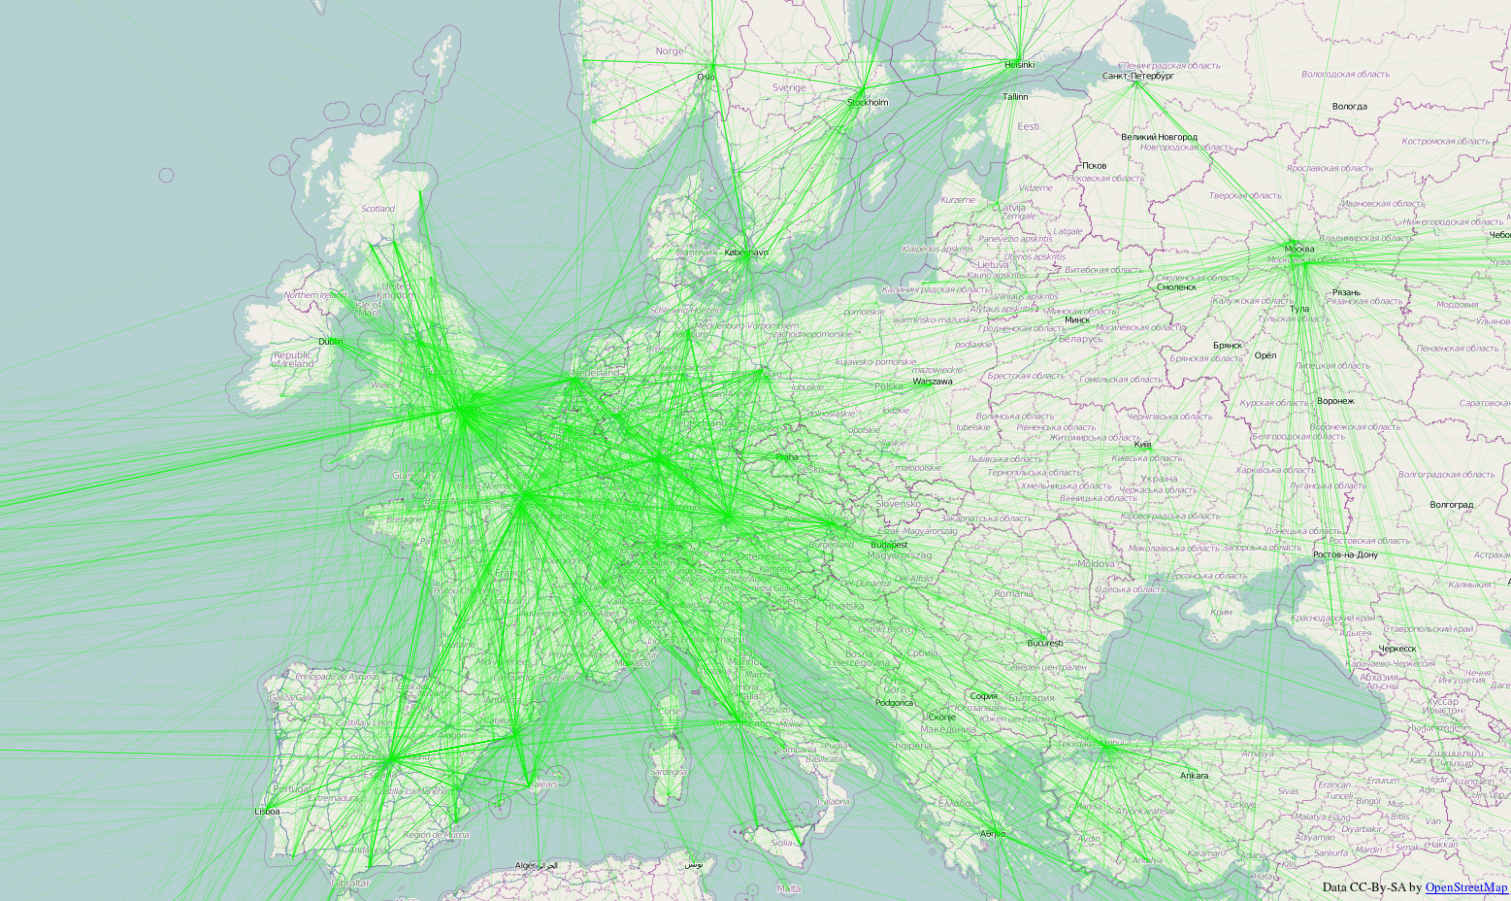
\includegraphics[width=0.6\textwidth, angle=0]{extending/figures/air/air_network_europe_osm} \end{center}

\createStandardInformation{todo}{todo}{todo}{\citet{GretherFuerbasNagel2013FlightTechnologyPROCEDIA,Grether2014PhD}}

% ##################################################################################################################
Options for the simulation of air- and rail-transport technology and passengers using \gls{matsim} are subject of this chapter. 
Overall travel times are often not that different between middle range rail and air transportation. 
Airports and railway stations are affected by capacity and opening time constraints. 
For passengers and goods, their geospatial location is an important property. 
Both modes, but especially air transport, are faced with hard capacity restrictions at fixed departure times. 

This chapter presents an approach, how \gls{matsim} can be applied to capture these constraints and how the interaction between a passenger demand and the constraints on the technology supply can be modeled. 
The public transit model of \gls{matsim} (Chapter~\ref{ch:pt}) is applied. %public transit vehicles and stops. 
Airports and aircraft are microscopically modeled the same way as bus stops and buses. 
Passengers are represented microscopically as multi-agent demand for air transportation. 
Their choice of transport mode, routes, and departure time is restricted by the capacity provided by the simulation model for air transport technology. 
The modeling of rail transport is based on teleportation. 
With appropriate data the modeling approach for air transport could also be applied to rail transport \citep{Quick2012BARailTraffic}.  

The modeling of technology and demand is sketched in Section~\ref{sec:air_rail_scenario}. 
On the basis of simulation results for a pure air transport model, rail transport is added and effects of mode choice are presented (Section~\ref{sec:air_rail_results}). 
Section~\ref{sec:air_rail_discussion} then interprets simulation results and highlights some modeling aspects that require further studies. 
Especially the choice set generation and plans removal algorithm of \gls{matsim} is discussed, that is also subject of Section~\ref{sec:future-of-scoring-function}. 
Modeling, results, and studies of this chapter present the highlights of \citet[][Chapter~6, pp.~119]{Grether2014PhD} where further details can be found in case of interest.   

% ##################################################################################################################
\section{Air Transport Scenario}
\label{sec:air_rail_scenario}
% ===========================================================================================
\subsection{Modeling \& Simulation of Air Transport Technology}
\label{sec:modeling-of-technology}
%
%\begin{figure}[t]
	%\begin{minipage}{0.5\linewidth}
				%\centering
			%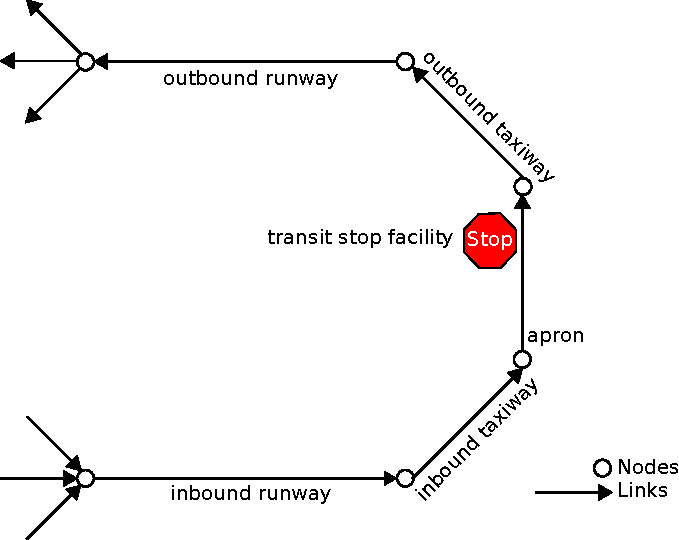
\includegraphics[width=0.9\textwidth]{extending/figures/air/sf_flight_model_airport.pdf}
		%\vspace{1.3cm}
%
			%%\scriptsize
			%\footnotesize
			%\begin{tabular}{@{}lrrr@{}}
				%Linktype & Count & Length [m] & Speed [km/h] \\
				%\hline
				%Runway   	& 2					& 1500		& $length \cdot c_{flow} $  	\\ % former value 220
				%Taxiway   	& 2					& 500		& 20  	\\
				%Apron   		& 1					& 500		& 20  	\\
				%\end{tabular}		
				%\vspace{1.4cm}
				%\caption{Airport layout and characteristics}
				%\label{fig:matsim_airport}
	%\end{minipage}
	%\begin{minipage}{0.5\linewidth}
		%\centering
		%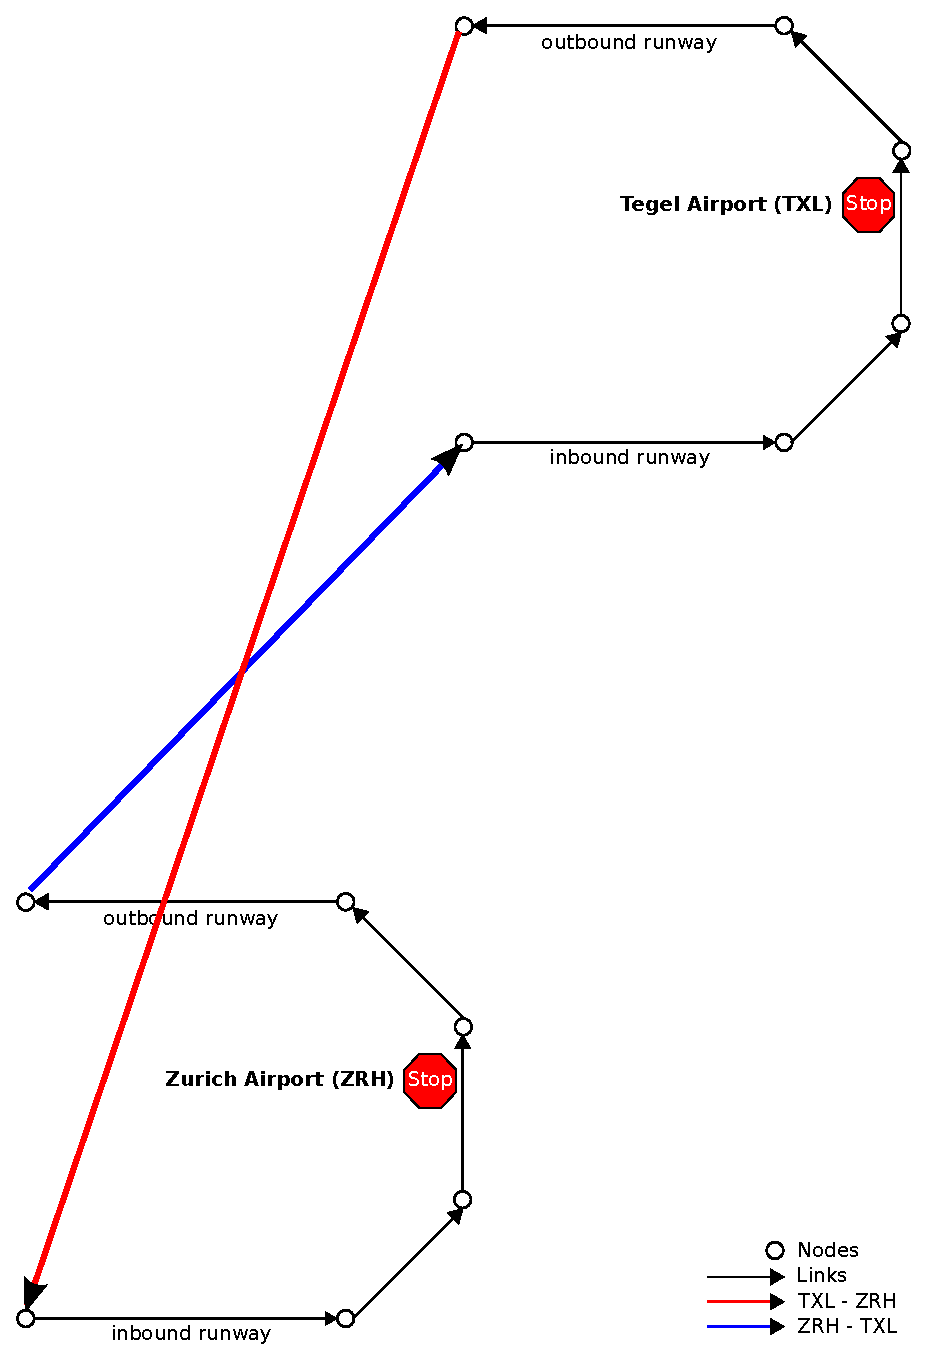
\includegraphics[width=0.9\textwidth]{extending/figures/air/sf_airport_network_no_slide.pdf}
		%\caption{Network layout}
		%\label{fig:matsim_network_model}
	%\end{minipage}
	%\caption{Layout of the air network, Source:~\citet{Grether2014PhD}}
	%\label{fig:air_network}
%\end{figure}
%
% ------------
\createfigure%
{Layout of the air network}%
{Layout of airports in the air transport network: In- and outbound runway are modeled by separate links that are connected by taxiways and a link representing the apron. There the transit stop facility is attached.}%
{\label{fig:air_airport}}%
{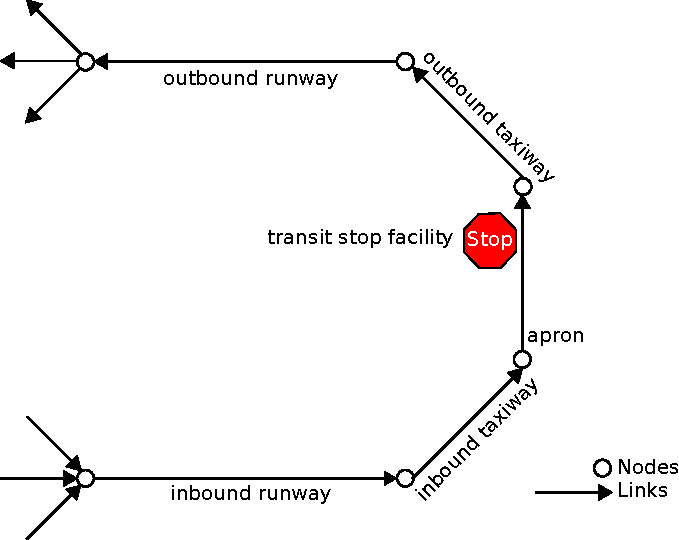
\includegraphics[width=0.8\textwidth]{extending/figures/air/sf_flight_model_airport.pdf}}%
{\citet{Grether2014PhD}}
% ------------
%
%\createtable%
%{Airport layout and characteristics}%
%{Airport layout and characteristics}%
%{\label{fig:matsim_airport}}%
%{%
%  \begin{tabular}{lrrr}
%		Linktype & Count & Length [m] & Speed [km/h] \\
%		\hline
%		Runway   	  & 2					& 1500	& $length \cdot c_{flow} $  	\\ % former value 220
%		Taxiway   	& 2					& 500		& 20  	\\
%		Apron   		& 1					& 500		& 20  	\\
%	\end{tabular}	
%}%
%{}
%
% ------------
\createfigure%
{Network layout}%
{Layout of airways in the air transport network: Each airport pair is directly connected by two airway links, one for each flight and direction. }%
{\label{fig:air_network_model}}
{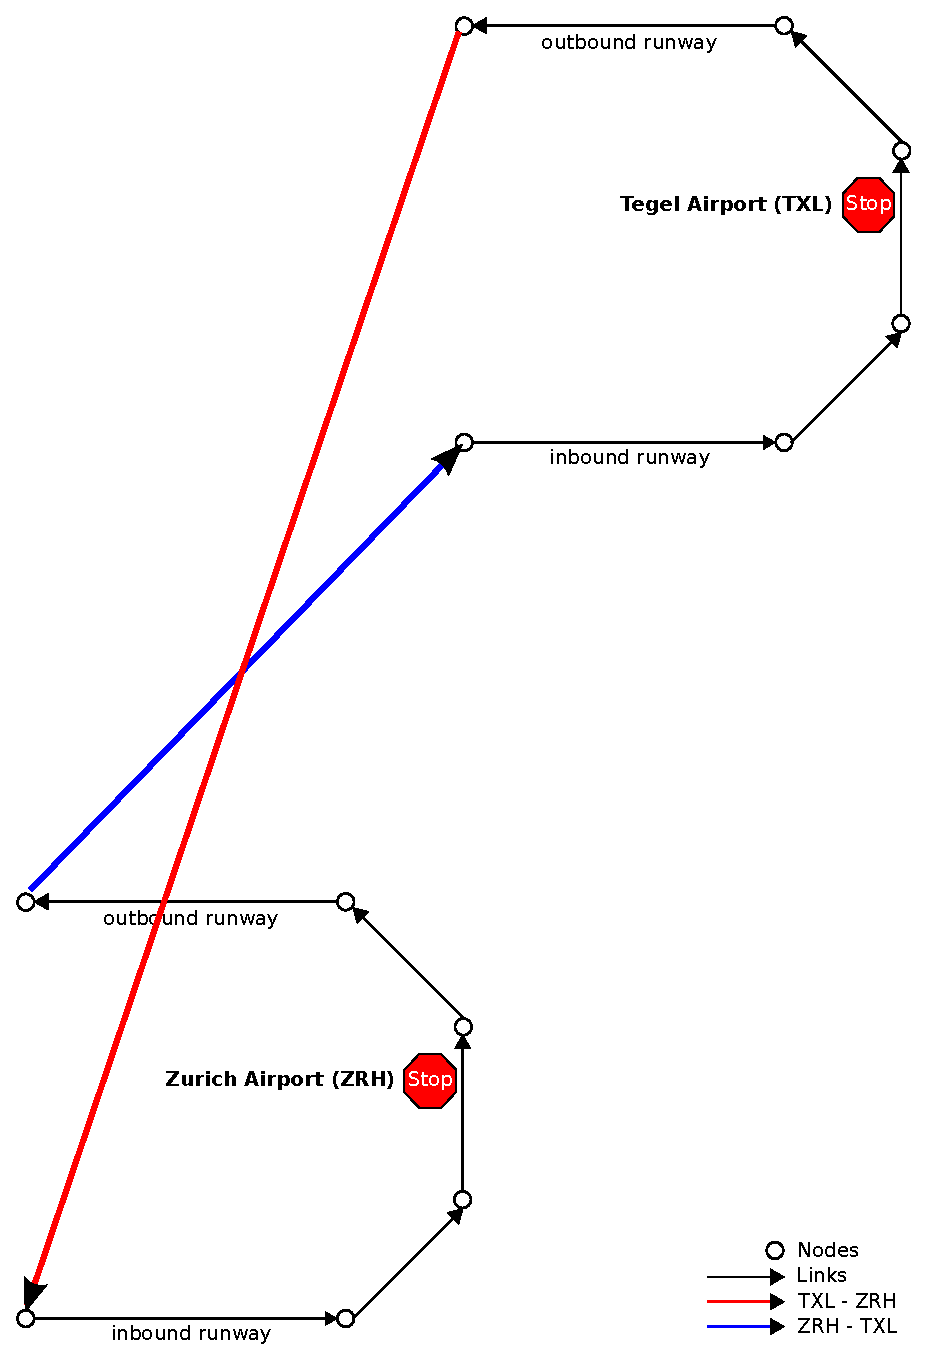
\includegraphics[width=0.8\textwidth]{extending/figures/air/sf_airport_network_no_slide.pdf}}%
{}
% ------------

%\mnote{OAG}
The air traffic technology model takes advantage of data provided by OAG Aviation\footnote{\url{www.oagaviation.com}, last access 08.08.2012}. 
Relevant data for schedule and network generation is excerpted from the September 2009 OAG data using all flights departing on a Tuesday, taking each specific flight number into account only once.
This may not always result in complete flight cycles, e.g.,\,when the outbound and inbound flight operate on different days of the week. 
Compared to using all flights of an entire week, the network may be incomplete, as certain destinations are only served on specific days.

%\mnote{Network}
The modeling of the air network aims at a simulation with \gls{matsim}.  
The network consists of airports, each showing an identical layout, and point-to-point connections in between. 
Every runway is solely used either for inbound or outbound flights with taxiways connecting the runways to the apron. The latter accommodates a transit stop, i.e.,\,the terminal, where flight movements originate and terminate (Figure~\ref{fig:air_airport}). 
Each airport pair is directly connected by airway links, one for each flight and direction of travel (Figure~\ref{fig:air_network_model}). 
The maximum speed on any of these links is calculated based on the distance and flight duration provided by OAG. 
Times for taxi, take-off, and landing are also taken into account, i.e.,\,the flight duration is reduced by the time needed from push-back to airborne before the maximum speed for an airway link is calculated.
Each flight has an individual link that could be interpreted as route, each possessing individual characteristics. 
Figure~\ref{fig:matsim_air_network_eu} shows parts of the network for European air traffic.
%
% ------------
\createfigure%
{European air network}%
{European air network with country borders in the background (country borders~\textcopyright~\url{openstreetmap.org})}%
{\label{fig:matsim_air_network_eu}}%
{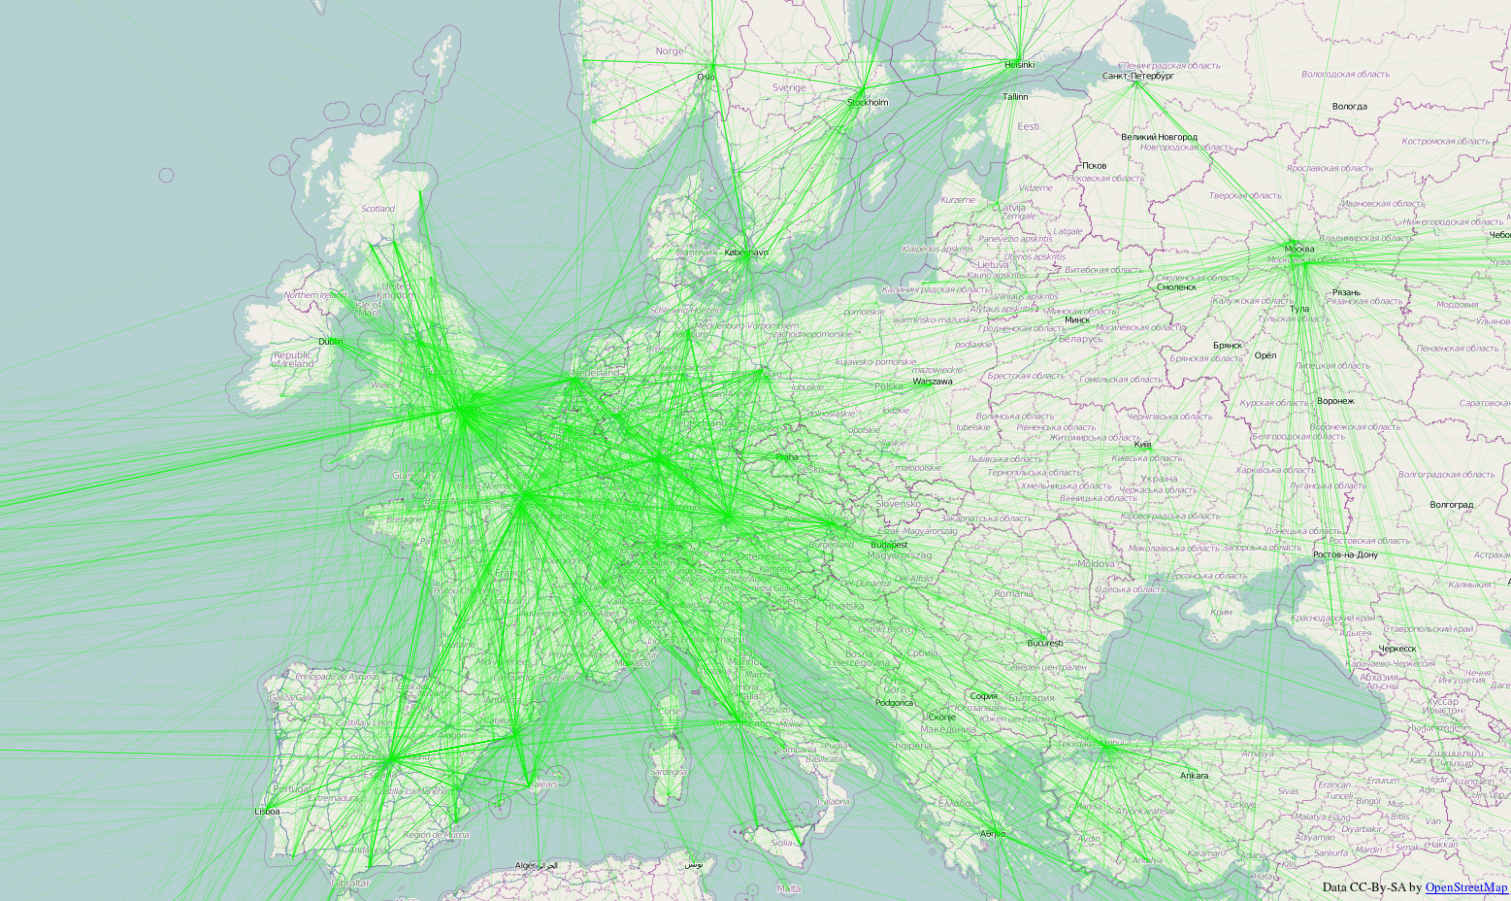
\includegraphics[width=0.99\textwidth, angle=0]{extending/figures/air/air_network_europe_osm.png}}%
{\citet{Grether2014PhD}}

% ------------

%\mnote{Flight Schedule}
The flight schedule is taken from the OAG data and translated to a \gls{matsim} transit schedule containing information about each line, route, and departure. 
For each airline that offers a connection between two airports, a transit line is generated. 
A transit route, which represents the route on the air traffic network, is created for each flight offered by this airline. 
%The route contains the links belonging to the airport representation plus the specific link for this flight connecting the airports' out- and inbound runway. 
Mutual interferences of aircrafts en-route are not included in the studies presented in this chapter.
%Tab.~\ref{tab:number_of_flights} lists the number of (not included) airports, direct origin-destination (O-D) connections and flight movements for three different area pairs.

%\mnote{Vehicles}
To represent individual aircraft in the simulation, transit vehicles are created on the basis of OAG data. 
IATA aircraft codes, operating airlines, and seating capacities are reflected in the respective aircraft representation for every flight. 
Information about boarding times, i.e.,\,passenger flow per door over time, is not available, but could be set for each aircraft type. 
One aircraft per flight is generated, thus delays resulting from a delayed incoming aircraft are not modeled.
Accordingly, no aircraft rotations and vehicle trip chains are implemented for the time being. 
The maximum velocity of each aircraft is set to twofold sonic speed, since speed limitations are set for each airway link of the network. 

% ===========================================================================================
\subsection{Passenger Demand}
%\mnote{Passengers, Synthetic Population}
As soon as you have modeled the technology side of air transport, you can start to simulate a passenger demand. 
The passenger demand for trips in Germany created and used for the results of this section is based on \gls{od} data of DESTATIS 
\footnote{\url{destatis.de}, Fachserie 8 Reihe 6, last access 10.09.2012}.
% 
For each \gls{od} pair and trip a virtual person is created.
Each virtual person performs two activities, one at the origin and the other at the destination airport. 
Both activities are of same type, thus time spent performing both activities is accumulated before it is evaluated by the utility function according to Section~\ref{sec:charyparnagel}. %equation (\ref{eq:utility_v_perf}). 
A typical duration, $t_{typ,q}$, of 21\,hours is set for this activity type. 
The time virtual persons arrive at the origin airport and start waiting for a connection is drawn randomly from a uniform distribution in 04:00 to 18:00, UTC. 
This reflects estimated typical opening hours of airports in Europe.
No other time constraints are set, thus the only incentive for virtual persons is to reduce overall travel time and maximize time spent at the activity. 
In between the two activities a flight leg is scheduled, connecting origin and destination.
As is common, the demand does not specify if a direct flight from O to D is chosen or the virtual person is on a route containing one or more transfers.
The synthetic population contains 51\,832\,virtual persons, 1\,550\,trips from the original data are neglected as origin and destination are equal. 
%

% ##################################################################################################################
\section{Simulation Results}
\label{sec:air_rail_results}
% ===========================================================================================
\subsection{Air Transport}
%\mnote{Parameters}
As scenario for air transport technology, a model with Europe to world wide coverage is used. 
Together with the synthetic population it serves as input for the simulation.
%model with no delays and no effective runway capacity restrictions 
%from 
%\technologyCite~is used.
The assignment of concrete flights to the desired \gls{od} connection, i.e.,\,the passenger routing, is calculated by the default public transit routing module of \gls{matsim}.

%\mnote{Simulation Runs}
Each simulation is run for 600\,iterations.
In each iteration, 10\,\% of the virtual persons may shift their departure time randomly within a 2\,hours interval.
Another 10\,\% may seek a new route, i.e.,\,a connection between origin and destination. 
Each passenger chooses out of a set of 5\,plans using an \gls{mnl}.
The outcome is stable after 500\,iterations, thus departure time choice and routing are switched off. 
For another 100\,iterations only the \gls{mnl} is used by the passengers to select a plan. 
%
% ------------
\createfigure%
{Passengers in aircraft and available seats over time in Germany}%
{Passengers in aircraft and available seats over time in Germany: At any time there are more seats than passengers. Air transport only scenario based on O-D data for Germany, iteration 600}%
{\label{fig:2009_passengers_seats}}%
{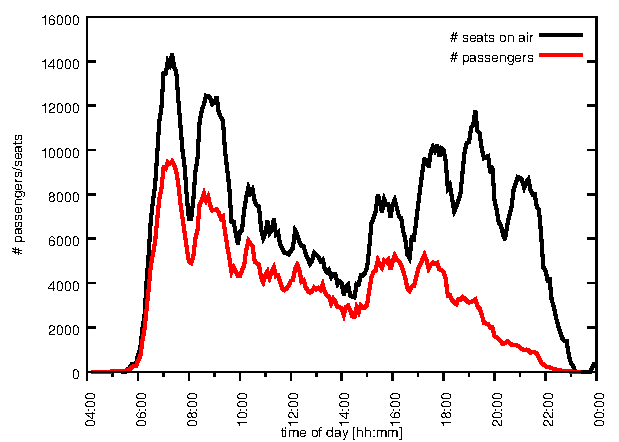
\includegraphics[width=0.99\textwidth, angle=0]{./extending/figures/air/in_vehicle_histogram_flight_1876_it_600.pdf}}%
{}

% ------------

Results are then taken from the output of the 600th iteration. 
Filtered by flights in Germany, Figure~\ref{fig:2009_passengers_seats} depicts passengers in aircraft (red) and seats (black) therein over time of day
and reveals the tendency of passengers to depart early. 

Some passengers fail to reach their destination, they get stuck.   
This is considered unrealistic, as only trips within Germany are modeled, which are usually completed within a few hours without any requirement for an overnight stay at an airport. 
320\,passengers get stuck at the end of the day. 
Getting stuck is not a consequence of a general lack of seats: at any time of day, there are more seats than demand.  
%
There are many reasons why stuck passengers can arise in such a situation.
%
Further analysis of the simulation results leads to the following insights for the $c_{lineswitch} = 0$ scenario:
\begin{compactitem}
\item 92\,passengers are stuck because there is no seat, and there is no other flight by the same airline later during the day to which they would be shifted otherwise.
\item 228\,passengers are stuck at an airport because there is no connection after their departure time 
	between that airport and their destination airport. 
\end{compactitem}

Neither departing early nor getting stuck are behavioral aspects explicitly modeled.  

% ===========================================================================================
\subsection{Adding an Alternative Mode}
%\mnote{Simulation Setup}
To gain further insights, in the following a slightly different simulation setup is applied. 
%The additional cost for each transfer is fixed to $c_{lineswitch} = 0$ and has no influence on the model. 
A second option for mode choice is added. 
Each virtual person can now choose between the micro-simulated air transport options and an alternative mode. 
The alternative mode has no capacity restrictions. 
Furthermore, passengers that travel with the alternative mode can start directly at their randomly selected departure time. 
The travel time, $tt$, is computed by the microsimulation with an estimation of the beeline distance between the \gls{od} pair $d$ and a velocity $v$, i.e.,\,$tt = d / v$.  
This velocity is varied in several simulation runs, i.e.,\,$v \in \{100, 150, 200, 250, 300 \} [km/h]$. 
If the alternative mode is chosen, the (dis-)utilities for traveling in the scoring are calculated accordingly.  

%Each person in the synthetic population obtains a second plan that uses the alternative mode. 
With this population the simulation is again run for 600\,iterations. 
Like in the previous simulations 10\,\% of the virtual persons may shift their departure times while another 10\,\% seek a different route between origin and destination in the air transport network. 
Additionally, further 10\,\% of virtual persons may change mode, i.e.,\,they can switch between the air traffic mode and the alternative mode. 
After 500\,iterations all choice modules are switched off, thus for the last 100\,iterations the logit model is used by passengers to select one of their plans. 

Simulation results for the 600th iteration show that the increasing speed of the alternative mode affects the modal split.  
While for a $v = 100 \, km/h$ the alternative mode is chosen by 1.2\,\% of the passengers, a mode alternative with a speed of 300\,kilometers per hour attracts 15.69\,\% of travelers. 
The number of stuck passengers for the alternative mode with $v = 100$\,kilometers per hour is remarkably reduced from approximately 320 to 67. 
Higher speeds of the alternative mode further reduce the number of stuck passengers. 
Slow speeds of the alternative mode implicate a dominance of the air transport mode. 
If there is a seat on a flight, travelers receive a higher score than by traveling on the alternative mode. 
However, travelers risk to get stuck, which can be hard to analyze and interpret. 
Further, it is an open issue of the implemented algorithm: If the number of plans per traveler exceeds a threshold of 5, the plan with the lowest score is removed from the plan database. 

% ------------
\createfigure%
{Results with random selector for plan removal, iteration 600.}%
{Passengers waiting for a flight or traveling by plane or by the alternative mode over time of day. 
Air transport and alternative mode scenario for Germany, iteration 600. Results with random selector for plan removal.}%
{\label{fig:2009_leg_histogram_modes_psl}}%
{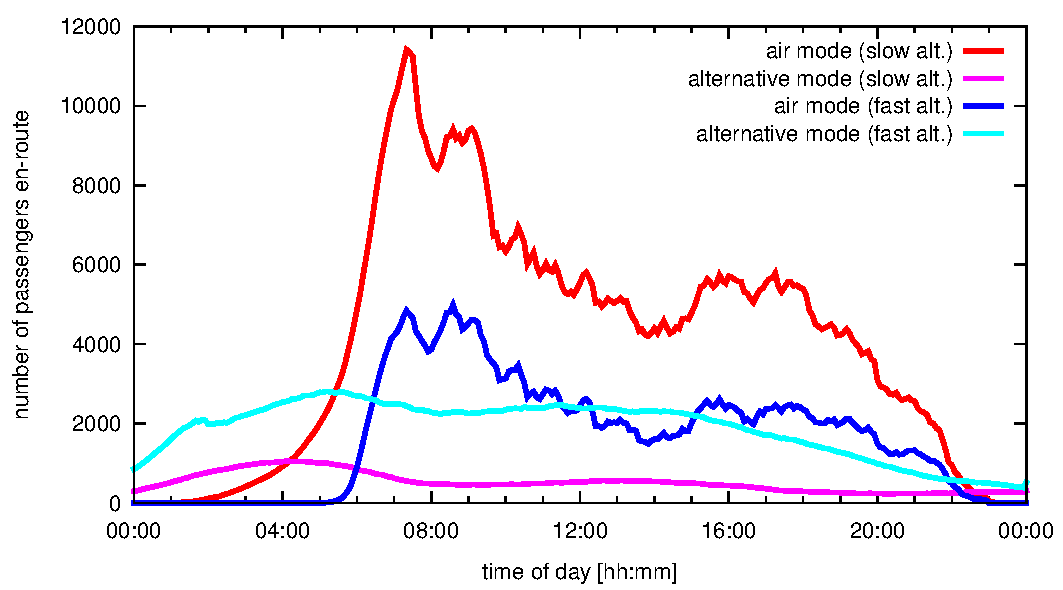
\includegraphics[width=0.99\textwidth, angle=0]{./extending/figures/air/leg_histogram_improved_flight_train_en_route_1893_1897_it_600.pdf}}%
{\citet{Grether2014PhD}}

% ------------
%
\createtable%
{Results with random selector for plan removal, iteration 600. Modal split for different speeds of the alternative mode}%
{Modal split for different speeds $v$ of the alternative mode. % 
Air transport and alternative mode scenario for Germany, iteration 600. %
Results with random selector for plan removal. % 
}%
{\label{tab:2009_results_train_modal_split_psl}}%
{%
  \begin{tabular}{@{}l|ccc|ccc@{}}
		$v [km/h]$	& \# air mode  & \# alt.~mode & \# stuck & air mode[\%]  & alt.~mode[\%] & stuck[\%] \\
		\hline 
		100 & 49280 & 2551 & 1 & 95.08 & 04.92 & 00.00\\	%1893 & 600
		150 & 44835 & 6996 & 1 & 86.50 & 13.50 & 00.00\\	%1894 & 600
		200 & 39929 & 11902 & 1 & 77.04 & 22.96 & 00.00\\	%1895 & 600
		250 & 34332 & 17499 & 1 & 66.24 & 33.76 & 00.00\\	%1896 & 600
		300 & 27270 & 24562 & 0 & 52.61 & 47.39 & 00.00\\	%1897 & 600
	\end{tabular}
}%
{}

Instead this deterministic removal of plans a probabilistic algorithm can be implemented, e.g.,\,plans for removal can be selected based on a path size logit model. 
With this modification the simulation runs are repeated. 
%with the same setup as for the runs that includes the alternative mode. 
Figure~\ref{fig:2009_leg_histogram_modes_psl} shows the resulting travel patterns over time for alternative modes at speed 100\,kilometers per hour and 300\,kilometers per hour.  
The distribution of travelers on the alternative mode over time of day is quite homogeneously. 
The speed increase of the alternative mode attracts more passengers. 
This is reflected by the modal splits in Table~\ref{tab:2009_results_train_modal_split_psl}. 
At most one passenger gets stuck at the end of day. 

\createtable%
{Results with random selector for plan removal, iteration 600. Simulation results including an alternative mode at different speeds $v$}%
{%
Error calculations for different speeds $v$ of the alternative mode. % 
Air transport and alternative mode scenario for Germany, iteration 600. %
Results with random selector for plan removal. % 
}%
{\label{tab:2009_results_alternative_mode_psl}}%
{%
  \begin{tabular}{@{}l|cccc@{}}
			$v [km/h]$ & $\sigma^2$ & $\sigma$ & mean rel error  & stuck \\
\hline
 $od_{transfer} - od_{direct}$ &  12640 & 112 & 1.75 & - \\
 \\
 100	& 10367 & 102 & 0.35 &  1 \\	% 1893 & 600
 150	& 13820 & 118 & 0.43 &  1 \\	% 1894 & 600
 200 & 18651 & 137 & 0.56 &  1 \\	% 1895 & 600
 250 & 25291 & 159 & 0.68 & 1 \\	% 1896 & 600
 300 & 36059 & 190 & 0.76 & 0 \\	% 1897 & 600
		\end{tabular}
}%
{}

The simulation results are further compared with the data of DESTATIS that serves as basis for the virtual population.  
The synthetic population is generated based on \gls{od} pairs that may contain transfers ($od_{transfers}$), 
while other DESTATIS data directly counts the number of passengers on actual direct flights ($od_{direct}$). % (2.2.1).
The latter is used to evaluate the accuracy of the model.
For comparison, the number of passengers on direct flights is calculated for each \gls{od} pair ($sim_{direct}$) from the simulation results.
Based on these data sets, the mean square error and the mean relative error are calculated\footnote{
The mean square error $\sigma^2$ is computed as
	$\sigma^2 = \frac{\sum_{i \in OD} (sim_{direct}(i) - od_{direct}(i))^2}{|OD|} \, , $
whereby $|OD|$ denotes the number of \gls{od} pairs, $sim_{direct}(i)$ the simulated passengers on a direct flight between the \gls{od} pair $i$, and $od_{direct}(i)$ the same, but retrieved from data.  
With the same values, the (unsigned) mean relative error for each \gls{od} relation is calculated as
$
\mbox{mean rel error} = \frac{\sum_{i \in OD} |(sim_{direct}(i) - od_{direct}(i))|/ od_{direct}(i)}{|OD|}.
$
}. 

Table~\ref{tab:2009_results_alternative_mode_psl} shows the outcome of these calculations. 
The first line contains the comparison of two sets of input data from DESTATIS\footnote{In the calculation, $sim_{direct}$ is replaced by $od_{transfers}$.}. 
This serves as reference as it would assume that all demand is served by direct flights.
All simulation runs explain the data better than that reference.
Mean square error and variance increase with the speed $v$ of the alternative mode.  
This is plausible as the demand only covers air transport trips. 

% ##################################################################################################################
\section{Interpretation \& Discussion}
\label{sec:air_rail_discussion}
The alternative mode can be interpreted as mixture between train, bus, or car connection availability. 
Clearly, the results hinge at the assumption that the alternative mode is always available and not capacity restricted.  
All passengers on the alternative mode face the same travel speed. 
This assumption is too coarse for the presented scenario. 
E.g., average speed and temporal availability of train connections depends on the \gls{od} pair. 
In principle, the alternative mode could be refined by inclusion of \gls{od} pair dependent average speed data. 
Alternatively, train, bus, and car can be simulated explicitly, featuring capacity restrictions and mutual interactions. 
For illustration of the overall modeling approach, however, a homogeneous velocity for the alternative mode seems to be more appropriate. 
%\mnote{Effects}
The effects evoked by the availability of the alternative mode are illustrative. 
The data for the demand provides \gls{od} pairs for air transport, but not for car, train or bus trips.  
For more plausible interpretations, further data for demand on other modes is required. 

%\mnote{Extent}
All the presented modeling approaches explain the routing of passengers in more detail than it can be solely retrieved from the input data.  
Most passengers use a direct connection, which is highly plausible considering the geospatial extent of the demand.  
Flying within Germany is often not worth it, if the connection includes a transfer. 
Then, empirically it is faster to travel by train, car, or bus. 
To gain further insights, the geospatial extent of the modeled demand could be increased which hinges at the availability of data not on the overall simulation approach. 

%\mnote{Time Structure}
Passengers are modeled without explicit desired departure or arrival times. 
The input data for this study does not contain any information about time distribution. 
The simulation approach can capture such individual time constraints.  
With some more data, the information can be added without big effort. 
This would resolve some of the presented problems concerning departure time choice. 

%\mnote{Stuck}
Passengers getting stuck are considered as not desired artifact of the simulation. 
Without the alternative mode, the only available transport mode is a capacity restricted flight connection that is served in discrete, irregular time intervals. 
The number of stuck passengers is higher than for the simulation runs with the alternative mode. 
Passengers get more likely stuck on \gls{od} pairs where the demand excesses seat capacity. 
This may have model extrinsic and intrinsic reasons. 

%\mnote{Extrinsic Stuck}
The quality of the simulation model's outcome hinges at the data available.  
For older studies of the air transport passenger demand, DESTATIS data for 09-2011 were used 
The air transport technology model, however, was created on a 09-2009 flight schedule.  
The number of starts of flights within Germany increased slightly between 2009 and 2011~\citep[][p.~23]{DLR2011Luftverkehrsbericht}. 
Assuming that the number of available seats is increased accordingly, the simulation model provided too little capacity, at least on certain \gls{od} pairs. 
As result, the number of passengers that had not reached their destination but got stuck was much higher.  
With the availability of 09-2009 DESTATIS data, the overall quality of results increased.  
The replacement of the 2011 data by 2009 data reduced the number of stuck passenger significantly, from around 1500 to 350\,travelers. 

Data is provided on a monthly basis, while the time horizon of the simulation model is one day. 
The number of trips per day is retrieved on the assumption that trips are uniformly distributed over all days of a month.  
The remaining 350\,stuck passengers might be resolved by a more accurate distribution. 
Otherwise, a longer time horizon could be simulated\footnote{Note, that this requires some changes in the source code that may not be resolved by sole customizations of \gls{matsim}. Please ask the developers before running \gls{matsim} for a longer time horizon.}. 
This would also include flights that are not departing on a Tuesday. 
Possibly, travelers no longer get stuck. 

%\mnote{Intrinsic Stuck}
The problem of stuck passenger can be model-intrinsic. 
The algorithm that removes plans is apparently the pivotal point to avoid stuck passengers. 
Replacing the deterministic by the probabilistic formulation resolves most of the stuck passengers. 
The applied path size logit modeling approach seems to be feasible, but requires further studies for parametrization and interpretation. 
In general, it allows the generation of more heterogeneous choice sets, see also Section~\ref{sec:choicesets}. 
With the deterministic plan removal plans with a high score but similar structure dominate all other generated plans. 
In combination with capacity restrictions the lack of alternatives results in stuck passengers.  
All other approaches to simulate more heterogeneity discussed on the following should consider these effects.  

%\mnote{Time Structure and Prices}
In further studies departure time choice and cost structures can be refined. 
If there is only one, early, connection to a hub per day, departure times of some passengers might be too late to reach that connection. 
The random departure time mutation may not be able to find that connection for all passengers. 
This has been ruled out for the current setup but should be considered in further studies. 

Alternatively, it may be the case that passengers have a connection that works in theory, but they are "crowded out" by other passengers who arrive earlier at the gate.  
They would make it if either of them would take a different route.  
The current approach would not find such a solution, since passengers do not take into account the costs they impose on others, see~\citet{LaemmelFloetteroed2009KISysOptEvac} for an approach to take that into account.  
The real-world solution presumably would be to raise prices on congested seats until one or the other passenger re-routes. 
Currently, all passengers have homogeneous values of time.   
For a more meaningful price modeling, more heterogeneous attributes of passengers can be included. 
As the present model is based on sole \gls{od} data, it does not include such a process. 
In principle, other data, as e.g.,\,Lorenz curves and median incomes, can be merged with the \gls{od} data~\citep{KickhoeferEtAl2011PolicyEvaluationIncome}.  

%\mnote{Diversity Routing}
An alternative approach to improve heterogeneity is a router that generates a larger diversity of routes even for the same departure time.  
Such a router would be able to point a passenger to a route where seats are available without by itself knowing about seat availability.  
That approach would, however, not address the issue that some passengers might need to switch their path in order to allow others to obtain a feasible path. 
In~\citet{Graf2013Da}, a first prototype of such a router is tested in a different context. 
First tests for the flight model revealed only slight improvements. 
As more diverse routes are dominated by the direct connection, they are removed by the algorithm similar to routes on slow alternative modes. 
After this more general problem is solved, a more diverse routing should be reconsidered. 

% ##################################################################################################################
\section{Conclusion}
Overall, the results show that a microscopic, agent-based simulation of passenger demand for air transport is feasible. 
Most passengers are able to learn the constraints of air transport technology and arrive at their desired destination.

The modeling of technology is similar to the approach by~\citet{ClarkeEtAl2007AirNetworkSim}, the level of detail is, however, coarser. 
In the same way as~\citet{ClarkeEtAl2007AirNetworkSim}, further models for, e.g.,\,gates, taxiing, weather or airline operations can be added to the presented approach. 
As the open source code of \gls{matsim} comes with options for extension, more detailed models of the technology side hinge on the availability of data. 
In contrast, and going beyond~\citet{ClarkeEtAl2007AirNetworkSim}, passengers are captured at all stages of their trip. 
Further, passengers traveling on alternative transport modes can be simulated. 
The chapter discusses some open issues, that are considered more general and not specific to air transport systems. 
The advice to the interested user is to support the \gls{matsim} team in solving these more general questions first.  
Then, the model may help to get a more detailed picture of mid-distance travel patterns.

Clearly, potential applications of the proposed model depend on type and detail of included information. 
In general, application for policy planning allows a more detailed evaluation of the effects from mid-distance travel policies that includes consideration of mode alternatives. 
The approach could also be useful for private companies, planning flight-schedules and capacities on their connections. 
The impacts of these changes on customers can be assessed on a high level of detail. 

% ##################################################################################################################

